\subsection{Limitación de tensi\'on de entrada}

La tensión de entrada máxima del circuito está limitada principalmente por el slew rate slew rate y la saturaci\'on. 

\subsubsection*{Influenccia del slew rate en $V_{in_{max}}$}

Partiendo de:
\begin{equation}
\begin{cases}
SR = m\'ax\bigg\{\frac{ dV_{out}}{dt}\bigg\} \\
V_{in} (f, t) = V_{in_{max}} \cdot sin(2\pi f t) \\
V_{out} (f, t) = \rvert H(f)\rvert \cdot V_{in_{max}} \cdot sin(2 \pi f t)
\end{cases}
\label{srecs}
\end{equation}

Siendo $SR$ el slew rate, $V_{in}$ y $V_{out}$ las se\~nales de entrada y de salida respectivamente y $\rvert H(f)\rvert = V_{out}/V_{in}$ la ganancia del circuito.


\begin{equation}
\frac{dV_{out}}{dt} = \rvert H(f)\rvert V_{in_{max}} 2 \pi f cos(2 \pi f t)
\label{deriv}
\end{equation}

Maximizando la ecuaci\'on \ref{deriv} se obtiene que:

\begin{equation}
SR = m\'ax\bigg\{\frac{dV_{out}}{dt}\bigg\} = \rvert H(f)\rvert 2 \pi f V_{in_{max}} 
\label{max}
\end{equation}

Despejando de la ecuaci\'on \ref{max}:

\begin{equation}
V_{in_{max}}  = \frac{SR}{\rvert H(f)\rvert 2\pi f}
\label{vinmax}
\end{equation}

El valor de SR, para el c\'alculo te\'orico, fue sacado de hojas de datos del amplificador operacional LM833 de Texas Instrument\footnote{Hoja de datos del operacional LM833: https://html.alldatasheet.com/html-pdf/784648/TI1/LM833/52/1/LM833.html}. 
Se encontr\'o que $SR = 7 \frac{V}{\mu s}$. Reemplazando con este valor en la expresi\'on \ref{vin_max}, se obtiene que la tensi\'on de entrada m\'axima limitada por el slew rate es:

\begin{equation}
	V_{in_{max}}  = \frac{\left(17,36 \cdot 10^8 f^{4} - 1.37 \cdot 10^{16} f^{2} + 3.52 \cdot 10^{22}\right)}{f \sqrt{61,19 \cdot 10^5 f^{8} - 62,49 \cdot 10^{12} f^{6} + 2.45 \cdot 10^{20} f^{4} - 3.57 \cdot 10^{26} f^{2} + 1.70 \cdot 10^{32}}}		
\label{vin_max}
\end{equation}


\begin{figure}[H] %!ht
	\centering
	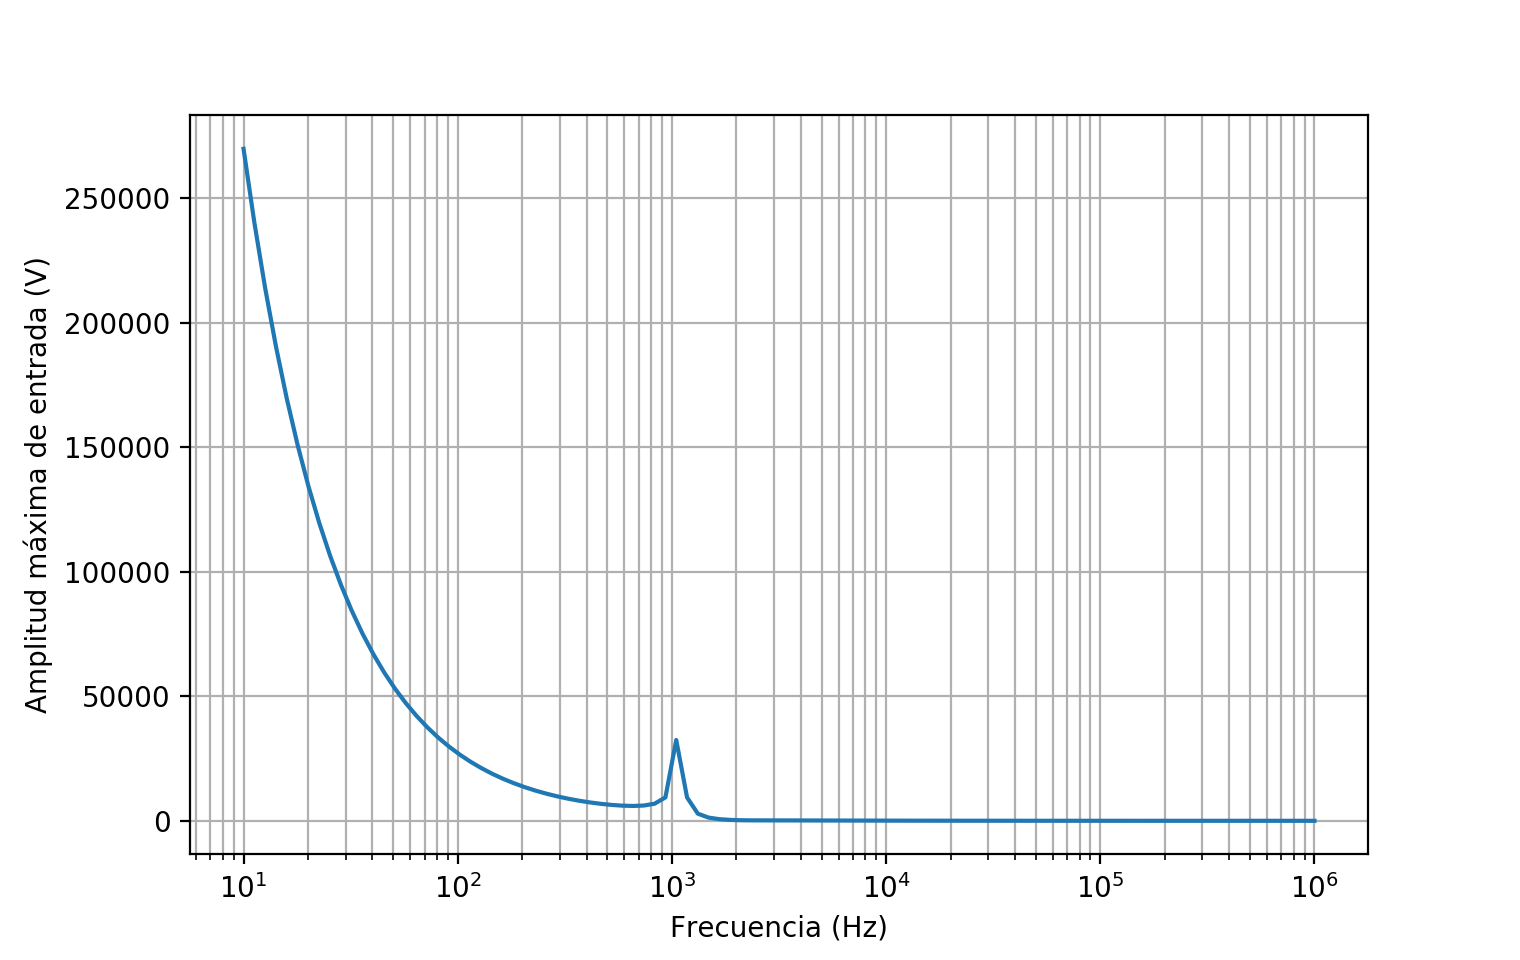
\includegraphics[width=10cm,height=10cm,keepaspectratio]{../EJ1/00GRAFICOS/vinmaxsr.png}
	\caption{Tensi\'on de entrada m\'axima limitada por slew rate.}
	\label{vinmaxsr}
\end{figure}

\subsubsection*{Influenccia de la saturaci\'on en $V_{in_{max}}$}
La tensi\'on pico a pico m\'axima de salida del amplificador operacional es llamada 
tensi\'on de saturasi\'on $V_{sat}$. Te\'oricamente, este valor es igual a $V_{CC}$. Dado que $V_{out} = \rvert H(s) \rvert V_{in}$:

\begin{equation}
V_{in_{max}} = \frac{V_{out_{max}}}{\rvert H(s) \rvert} = \frac{V_{sat}}{\rvert H(s) \rvert} = \frac{V_{CC}}{\rvert H(s) \rvert}
\end{equation}

Dado que en nuestro caso usamos $V_{CC} = \pm15V$, la expresi\'on que se obtiene es:

\begin{equation}
V_{in_{max}} = \frac{15V}{\rvert H(s) \rvert} 
\end{equation}

\todo{en ec anterior poner cuanto da numericamente}


\begin{figure}[H] %!ht
	\centering
	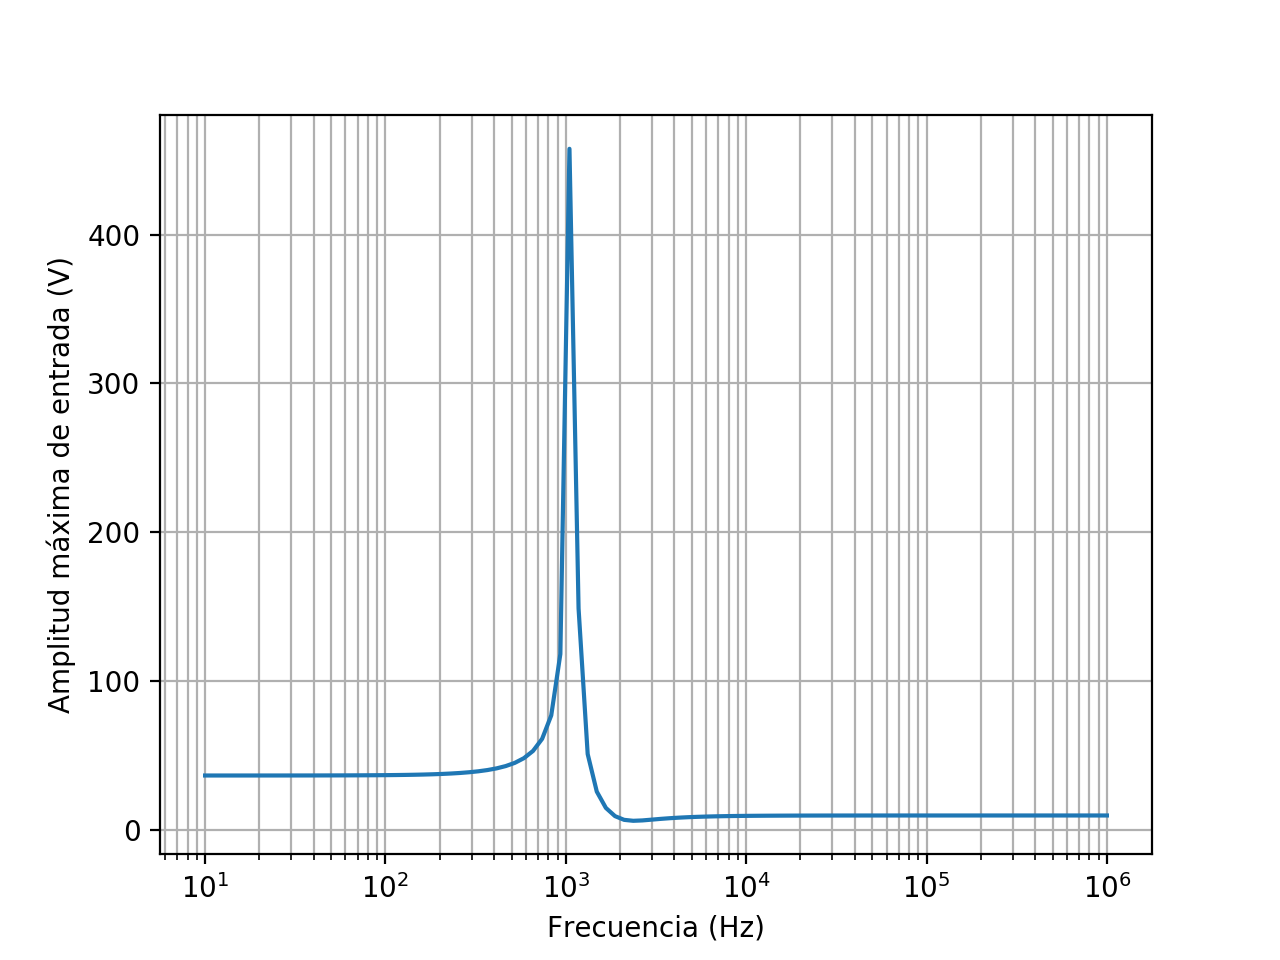
\includegraphics[width=10cm,height=10cm,keepaspectratio]{../EJ1/00GRAFICOS/vinmaxsat.png}
	\caption{Tensi\'on m\'axima de entrada limitada por saturaci\'on.}
	\label{vinmaxsat}
\end{figure}

\subsubsection*{Combinaci\'on del efecto de slew rate y saturaci\'on sobre la tensi\'on m\'axima de entrada}


\begin{figure}[H] %!ht
	\centering
	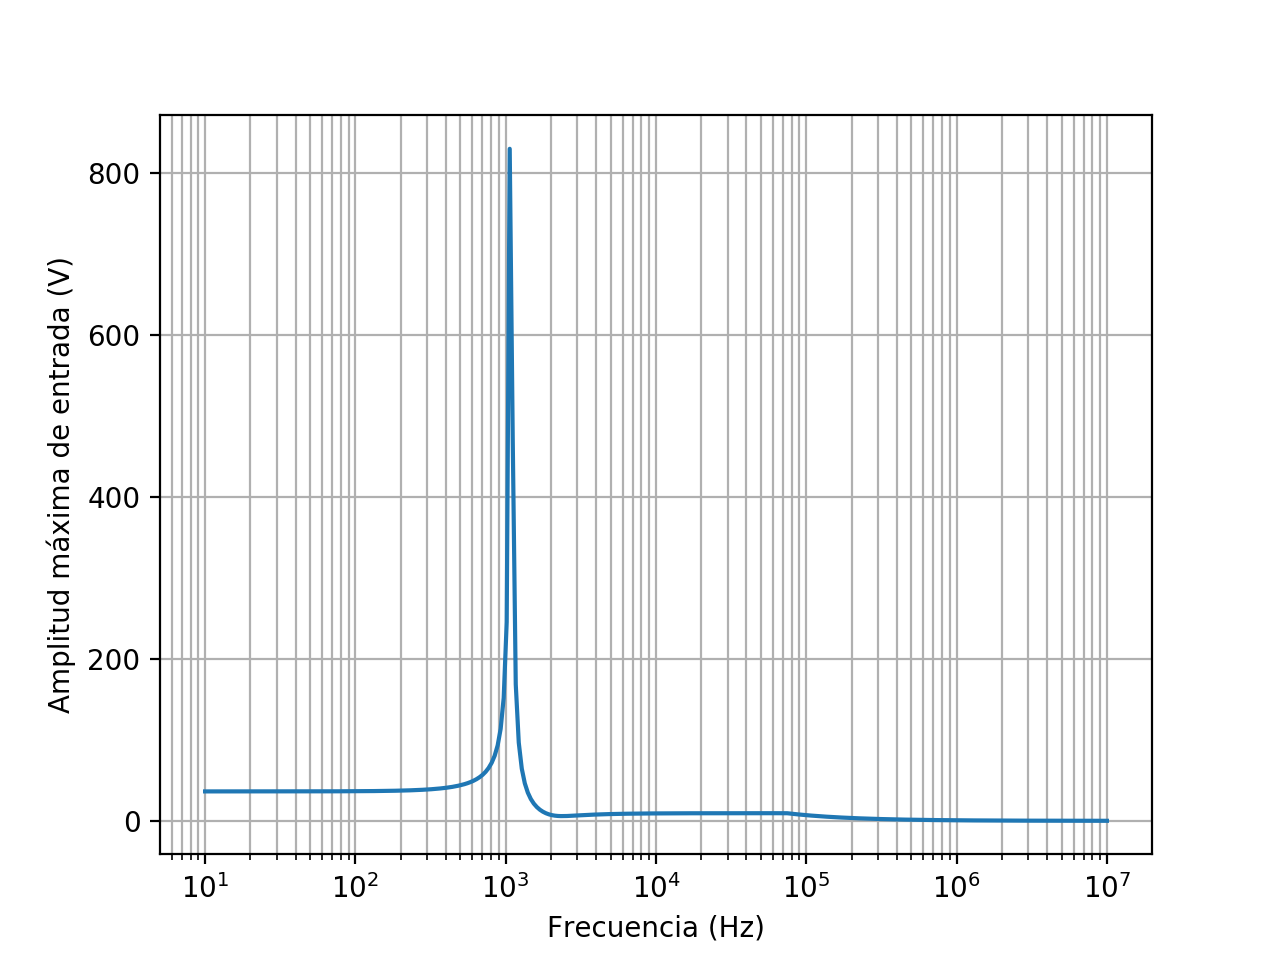
\includegraphics[width=10cm,height=10cm,keepaspectratio]{../EJ1/00GRAFICOS/vinmaxtotal.png}
	\caption{Tensi\'on m\'axima de entrada limitada por slew rate y saturaci\'on.}
	\label{vinmaxtotal}
\end{figure}

En el gr\'afico \ref{vinmaxtotal} se puede ver que la forma que presenta la curva correspondiente a la tensi\'on de entrada m\'axima al circuito respecto a la frecuencia, es inversa a aquella de la funci\'on transferencia. Esto se debe a que al tratarse de un high pass notch, donde hay ganancia de tensi\'on, disminuye la tensi\'on m\'axima de entrada ya que la misma puede saturar al superar la tensi\'on de Vcc. Cerca de la frecuencia del pico del notch, al haber mucha atenuaci\'on, la tensi\'on m\'axima de entrada aumenta enormemente ya que igual ser\'a atenuada al ingresar al cirucuito.